%-------------------------------------------------------------------------------
%                            BAB III
%               		METODOLOGI PENELITIAN
%-------------------------------------------------------------------------------
% \fancyhf{} 
% \fancyfoot[C]{\thepage}
\captionsetup[figure]{labelfont={normalfont}, textfont={normalfont}}

\chapter{METODOLOGI PENELITIAN}

\section{Tempat dan Waktu Penelitian}
Penelitian tugas akhir dilaksanakan di Laboratorium \textit{Strategic Risk Governance} (SRG) TDMRC USK, Banda Aceh. Adapun lokasi pengumpulan data lapangan mencakup Kecamatan Montasik (Desa Mata Ie dan Atong), Kecamatan Indrapuri (Desa Lam Ilie Mesjid dan Reukih Keupula), dan Kecamatan Darussalam (Desa Lambada Peukan). Pemilihan lokasi didasarkan pada representativitas wilayah tersebut terhadap aktivitas pertanian padi di Kabupaten Aceh Besar. Penelitian berlangsung selama enam bulan, dari Oktober 2025 hingga Maret 2026.

%-----------------------------------------------------------------------------%
% \section{Jadwal Pelaksanaan Penelitian}
% Adapun jadwal pelaksanaan penelitian ini dapat dilihat pada distribusi pada Tabel 3.1 dibawah ini.

% \begin{table}[h]
% \centering
%     \renewcommand{\arraystretch}{1.3}
%     \renewcommand{\arrayrulewidth}{0.3mm}
%     \setlength{\tabcolsep}{4pt}
%     \caption{Jadwal Pelaksanaan Penelitian}
%     \resizebox{\columnwidth}{!}{
%     \begin{tabular}{|c|p{4.5cm}|*{24}{c|}}
%         \hline
%         \multirow{2}{*}{No} & \multirow{2}{*}{\centering Kegiatan} & \multicolumn{24}{c|}{Bulan Ke -} \\ 
%         \cline{3-26}
%         & & \multicolumn{4}{c|}{Oktober} & \multicolumn{4}{c|}{November} & \multicolumn{4}{c|}{Desember} & \multicolumn{4}{c|}{Januari} & \multicolumn{4}{c|}{Februari} & \multicolumn{4}{c|}{Maret} \\ 
%         \hline
%         & & 1 & 2 & 3 & 4 & 1 & 2 & 3 & 4 & 1 & 2 & 3 & 4 & 1 & 2 & 3 & 4 & 1 & 2 & 3 & 4 & 1 & 2 & 3 & 4 \\ 
%         \hline
%         1 & Analisis Kebutuhan & \cellcolor{black} & \cellcolor{black} & \cellcolor{black} &  &  &  &  &  &  &  &  &  &  &  &  &  &  &  &  &  &  &  &  &  \\ \hline
%         2 & Studi Literatur &  & \cellcolor{black} & \cellcolor{black} & \cellcolor{black} &  &  &  &  &  &  &  &  &  &  &  &  &  &  &  &  &  &  &  &  \\ \hline
%         3 & Perancangan Sistem &  &  &  & \cellcolor{black} & \cellcolor{black} & \cellcolor{black} &  &  &  &  &  &  &  &  &  &  &  &  &  &  &  &  &  &  \\ \hline
%         4 & Rancang API &  &  &  &  &  & \cellcolor{black} & \cellcolor{black} & \cellcolor{black} & \cellcolor{black} & \cellcolor{black} & \cellcolor{black} & \cellcolor{black} & \cellcolor{black} & \cellcolor{black} & \cellcolor{black} &  &  &  &  &  &  &  &  &  \\ \hline
%         5 & Preprocessing Dataset &  &  &  &  &  &  &  &  &  &  & \cellcolor{black} & \cellcolor{black} & \cellcolor{black} & \cellcolor{black} & \cellcolor{black} & \cellcolor{black} & \cellcolor{black} & \cellcolor{black} &  &  &  &  &  &  \\ \hline   
%         6 & Implementasi \textit{Scheduler} &  &  &  &  &  &  &  &  &  &  &  & \cellcolor{black} & \cellcolor{black} & \cellcolor{black} & \cellcolor{black} & \cellcolor{black} & \cellcolor{black} & \cellcolor{black} &  &  &  &  &  &  \\ \hline
%         7 & Implementasi Sistem oleh Petani  &  &  &  &  &  &  &  &  &  &  &  &  &  &  &  &  &  &  & \cellcolor{black} & \cellcolor{black} & \cellcolor{black} & \cellcolor{black} & \cellcolor{black} & \cellcolor{black} \\ \hline
%     \end{tabular}
%     }
% \end{table}

%-----------------------------------------------------------------------------%

\section{Alat dan Bahan}
Alat dan Bahan yang digunakan dalam penelitian ini terdiri dari beberapa \textit{hardware} maupun \textit{software} yang dijabarkan sebagai berikut: 

\subsection{Perangkat keras}
Perangkat keras yang digunakan dalam penelitian ini adalah Laptop Lenovo ThinkPad X280 dengan spesifikasi \textit{Processor} Intel Core i5-8350U (4\-Core 8\-Thread) 3.60 GHz, RAM 16 GB DDR4, dan penyimpanan SSD 1 TB.

\subsection{Perangkat lunak}
Adapun perangkat lunak yang digunakan akan dijabarkan sebagai berikut:
\begin{multicols}{3}
\begin{itemize}
    \setlength\itemsep{0pt}
    \setlength\parskip{0pt}
    \setlength\parsep{0pt}
    \setlength\topsep{0pt}
    \setlength\partopsep{0pt}
    \item OS Arch Linux 6.18.33-1-lts
    \item OS Ubuntu Server 7.0.0-27-generic
    \item Visual Studio Code 1.104.1
    \item Flask 3.1.2
    \item Next.js 16.2.4
    \item MongoDB 8.0.13
    \item Gunicorn 26.0.0
    \item Ngrok 3.39.2
    \item Cron
    \item Postman
\end{itemize}
\end{multicols}

\section{Prosedur Penelitian}
Prosedur penelitian yang dilakukan terbagi menjadi beberapa tahapan yang dijelaskan pada Gambar \ref{alur_penelitian} di bawah ini. 
\begin{figure}[H]
    \centering
    
\includegraphics[width=0.70\linewidth]{image/bab3/bab_iii_alur.png}
    \caption{Diagram Alur Prosedur Penelitian}
    \label{alur_penelitian}
\end{figure}

\subsection{Survei kuesioner}
Survei kuesioner dilakukan untuk memperoleh data primer mengenai praktik pertanian padi di wilayah penelitian, meliputi jenis varietas yang digunakan, pola tanam, karakteristik lahan, serta persepsi petani terhadap pengaruh kondisi iklim terhadap kegiatan budidaya.

Perlu ditegaskan bahwa hasil survei tidak digunakan dalam \textit{preprocessing} data iklim. Tahapan \textit{preprocessing} sepenuhnya didasarkan pada karakteristik \textit{dataset} sebagaimana telah dijelaskan pada Bab II. Sebaliknya, hasil kuesioner dimanfaatkan sebagai dasar dalam penyusunan kalender tanam digital, mengenai identifikasi periode tanam, parameter iklim pengambilan keputusan tanam, serta kebutuhan informasi yang perlu disajikan oleh sistem. Dengan demikian, survei kuesioner berfungsi sebagai pendukung pengembangan fitur kalender tanam digital, sedangkan proses pengolahan data iklim dilakukan secara independen melalui \textit{pipeline preprocessing} yang akan dirancang.

\subsection{Kerangka kerja agile}
Penelitian ini mengadopsi pendekatan \textit{Agile Development} karena pengembangan sistem otomasi data iklim memerlukan fleksibilitas tinggi terhadap perubahan kebutuhan sistem, penyesuaian format \textit{dataset}, serta integrasi layanan. Pendekatan \textit{agile} memungkinkan proses pengembangan dilakukan secara bertahap dan iteratif sehingga setiap perubahan atau penyesuaian dapat diimplementasikan tanpa mengganggu keseluruhan sistem. Metode ini mendukung proses evaluasi berkelanjutan pada fitur \textit{preprocessing}, pengelolaan metadata, serta integrasi dengan kebutuhan analisis lanjutan dan model \textit{forecasting} tim \citep{jovanovic2020}.

Dalam implementasinya, penelitian dibagi ke dalam lima \textit{sprint} dengan durasi masing-masing 2 hingga 4 minggu. Setiap \textit{sprint} difokuskan pada pengembangan dan penyempurnaan fitur tertentu, seperti otomasi \textit{scheduler}, \textit{preprocessing} data iklim, integrasi RESTful API, serta pengelolaan metadata \textit{dataset}. Pada akhir setiap \textit{sprint}, dilakukan pengujian \textit{backend} dan evaluasi integrasi sistem untuk memastikan stabilitas, skalabilitas, dan kesiapan sistem sebelum melanjutkan ke tahapan berikutnya. Rincian pembagian \textit{sprint} dapat dilihat pada Tabel \ref{pembagian_sprint} di bawah ini.

\begin{table}[H]
    \centering
    \caption{Pembagian \textit{Sprint} dalam Pengembangan Sistem}
    \label{pembagian_sprint}
    % 1. Mengecilkan ukuran font
    \small 
    % 2. Mengurangi padding horizontal antar kolom (default biasanya 6pt)
    \setlength{\tabcolsep}{4pt} 
    % 3. Mengatur padding vertikal agar tetap ramping tapi tidak menempel
    \renewcommand{\arraystretch}{1.1} 
    
    % Menggunakan |c|l|l| untuk garis vertikal standar
    \begin{tabular}{|c|l|l|}
        \hline
        \textbf{Sprint} & \textbf{Fokus Pengembangan} & \textbf{Output Utama} \\
        \hline
        1 & Analisis kebutuhan & \textit{Product backlog} \\
        \hline
        2 & Perancangan dan implementasi \textit{frontend} & \textit{Prototype}, UI \textit{dashboard} \\
        \hline
        3 & Implementasi \textit{backend} dan RESTful API & \textit{Preprocessing endpoint} \\
        \hline
        4 & Implementasi \textit{smoothing} & Otomasi sistem \\
        \hline
        5 & Pengujian dan \textit{deployment} & \textit{System live} \\
        \hline
    \end{tabular}
\end{table}

Tabel \ref{pembagian_sprint} merincikan pembagian tahapan \textit{sprint} yang dilakukan dalam pengembangan sistem. Penjelasan mengenai rincian aktivitas dari setiap \textit{sprint} akan dijelaskan pada subbab di bawah ini.
 
\subsection{Analisa kebutuhan}
Sprint pertama adalah analisis kebutuhan, yaitu proses memahami spesifikasi sistem yang akan dikembangkan. Analisis mencakup identifikasi kebutuhan pengguna, tujuan penelitian, maupun \textit{tech stack} yang digunakan dalam membangun otomasi sistem pemrosesan data iklim. Diperlukan juga rancangan fungsional sistem meliputi pengambilan data iklim, \textit{preprocessing} data, dan penerapan metode \textit{smoothing}. Diperlukan juga rancangan non-fungsional meliputi aspek performa, keamanan, dan skalabilitas sistem.

Hasil dari analisis ini akan didokumentasikan dalam bentuk \textit{product backlog} mencakup rincian prioritas fitur, deskripsi teknis, dan perbaikan versi sebelumnya. Dokumentasi akan memastikan proses pengembangan berjalan secara terarah sesuai dengan kebutuhan teridentifikasi.

% \subsection{Studi literatur}
% Selanjutnya dilakukan studi literatur untuk meneliti berbagai teknologi dan metode dalam pemrosesan data iklim. Studi ini mencakup penelitian terdahulu mengenai manajemen sistem iklim, metode \textit{preprocessing} data, serta teknologi dalam pengembangan aplikasi berbasis web. Literatur meliputi jurnal ilmiah dan publikasi di mana membahas penerapan otomasi dalam pengolahan data lingkungan, terutama pada konteks prediksi iklim dan manajemen informasi iklim. Penelitian juga meninjau berbagai pendekatan dalam \textit{preprocessing} data iklim, teknik interpolasi, dan normalisasi data.

\subsection{Perancangan sistem}
Perancangan sistem mengikuti pendekatan \textit{client-server} melalui empat komponen, yaitu komponen utama, diantaranya \textit{frontend} berbasis Next.js sebagai \textit{interface}, \textit{backend} berbasis Flask RESTful API sebagai \textit{logic flow}, MongoDB sebagai penyimpanan data, dan alur pembersihan \textit{dataset}.

\begin{enumerate}[(a)]
    \item \textbf{Perancangan alur kerja sistem}
    \par \textit{Activity Diagram} dibuat untuk menjelaskan hubungan alur kerja anggota tim, dimulai dari pengambilan data iklim, pembersihan \textit{dataset} oleh Anggota 1, penerapan algoritma Holt-Winters oleh Anggota 2, hingga pelatihan model LSTM oleh Anggota 3. Adapun detail dijabarkan pada Gambar \ref{pembagian_tugas} di bawah ini.
    \begin{figure}[H]
    \centering
    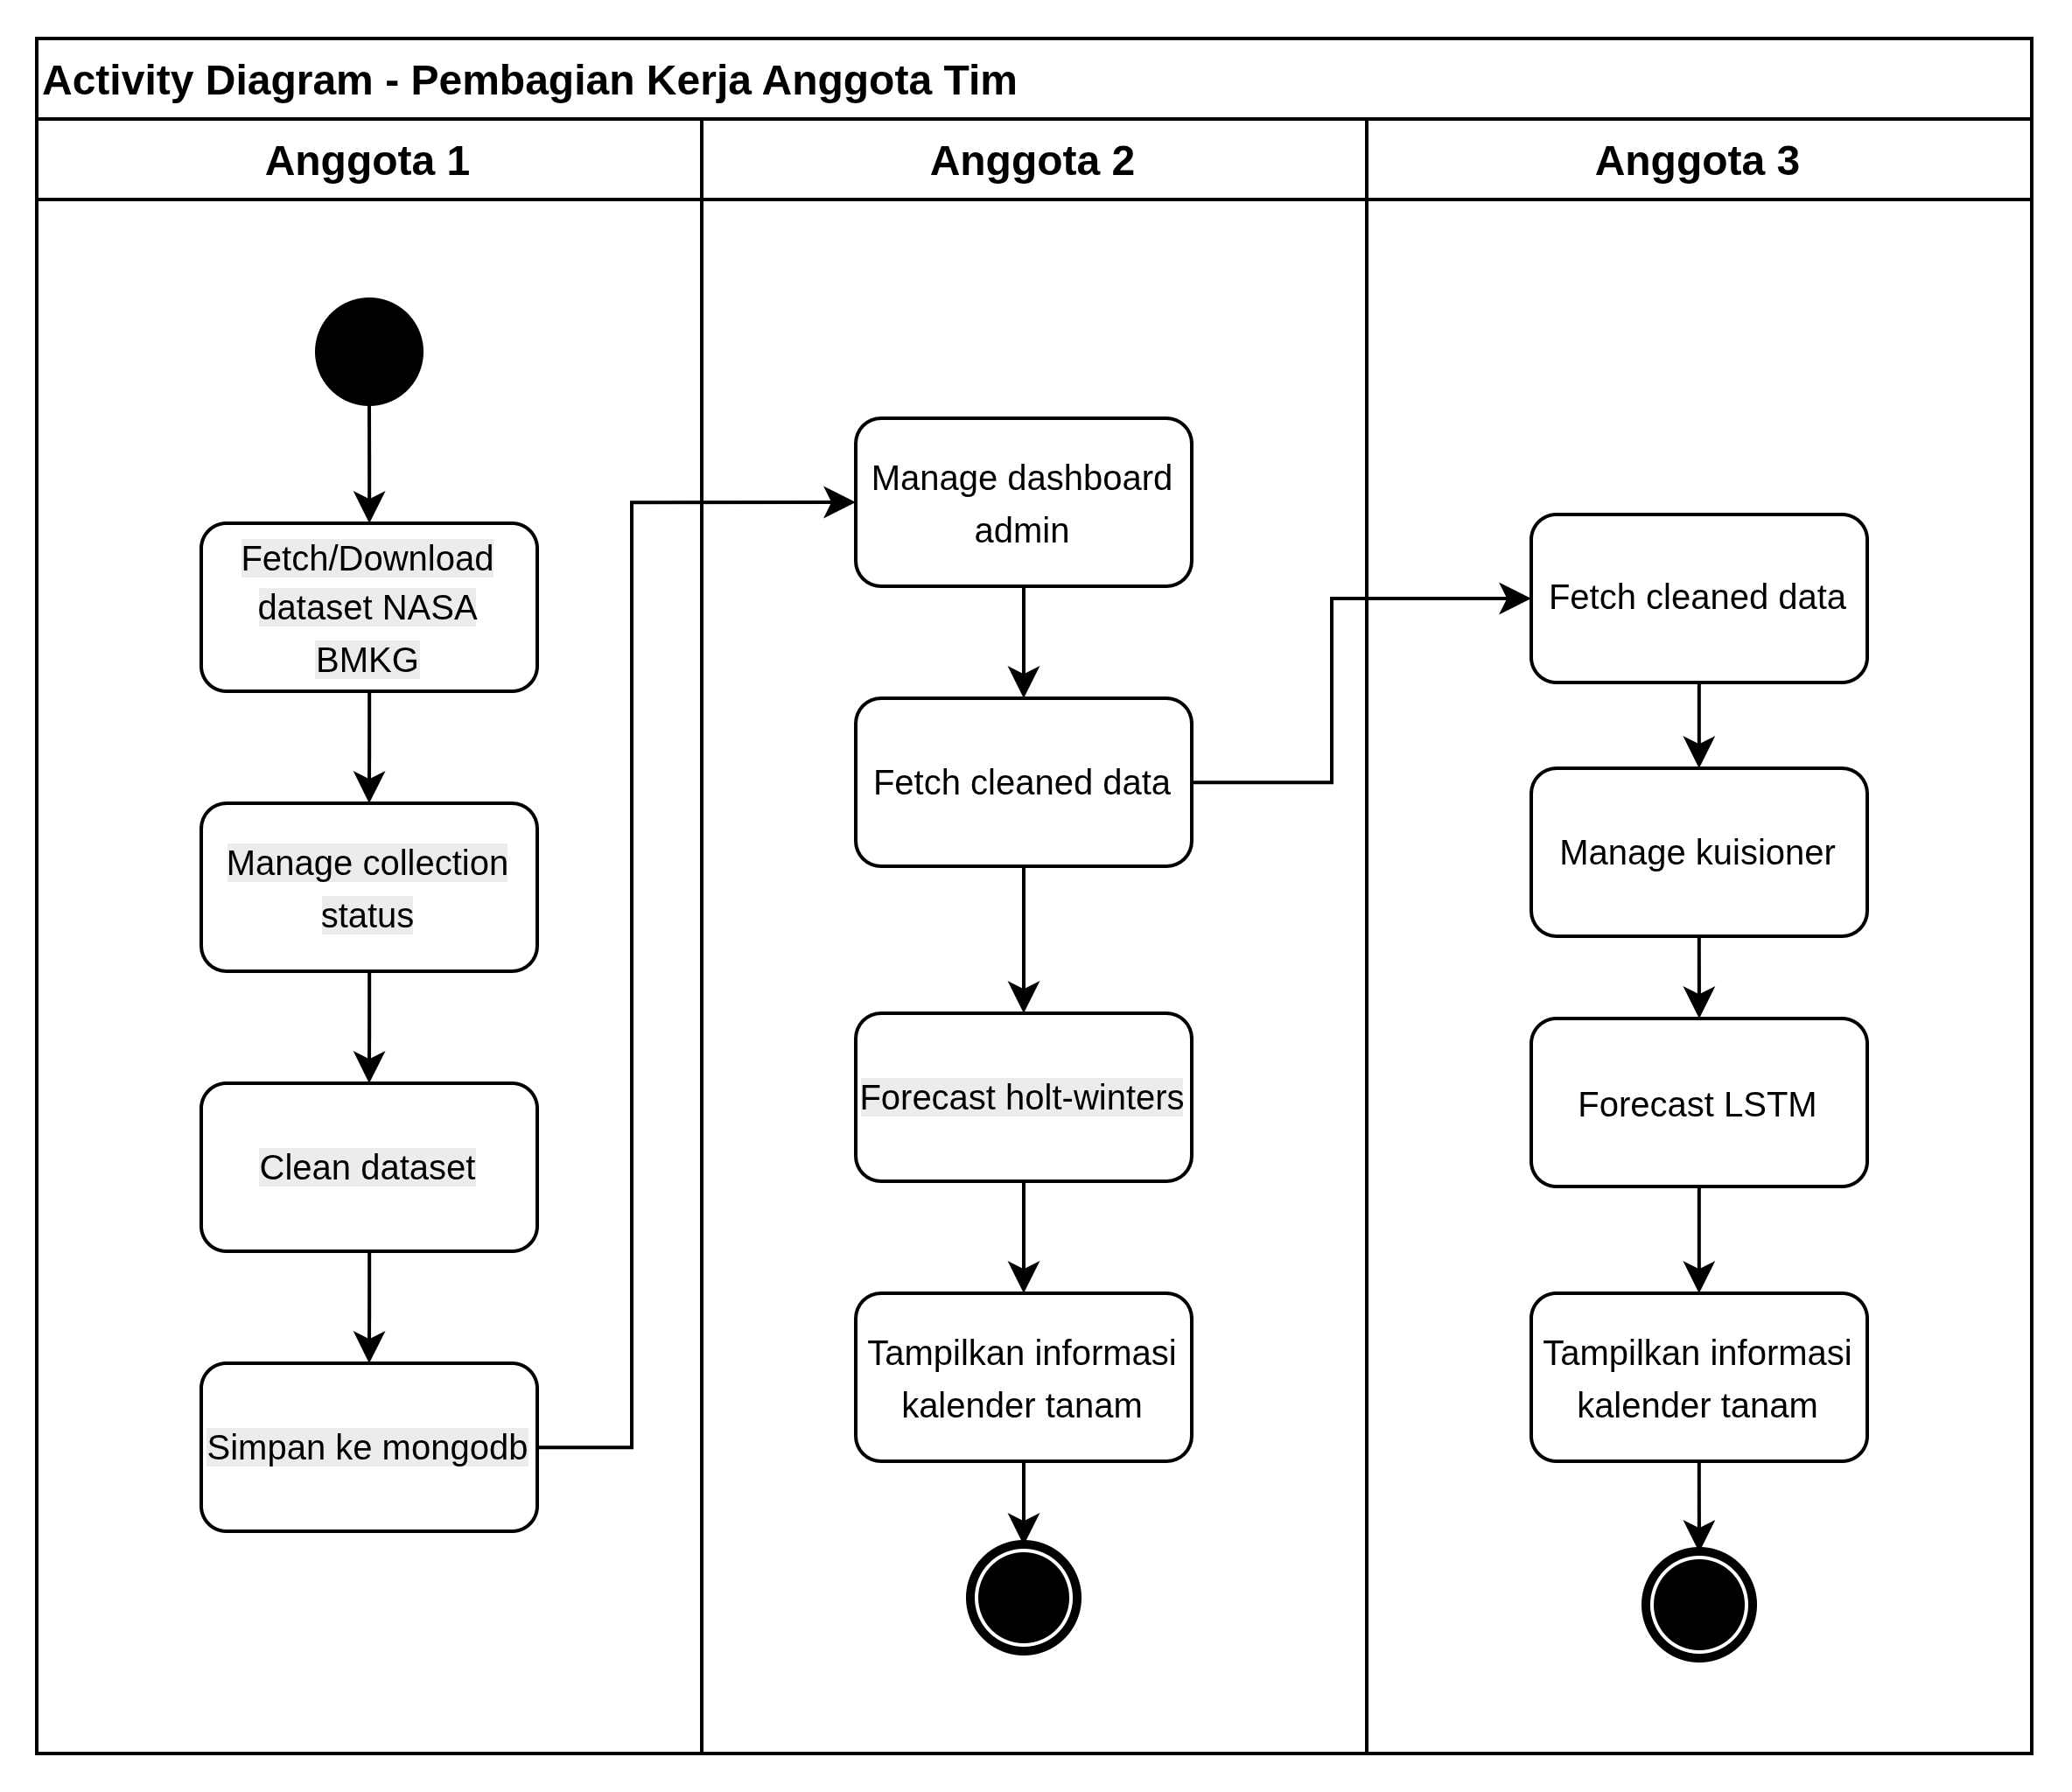
\includegraphics[width=0.6\linewidth]{image/bab3/activity_pembagian.png}
    \caption{\textit{Activity Diagram} Pembagian Tugas Anggota Tim}
    \label{pembagian_tugas}
    \end{figure}

    Pada penelitian ini, penulis merupakan Anggota 1 yang bertanggung jawab dalam proses \textit{data acquisition}, \textit{data cleaning}, dan \textit{data integration}, seperti yang dijelaskan pada \textit{flowchart} Gambar \ref{fig:flowchart_1}.
    \begin{figure}[H]
    \centering
    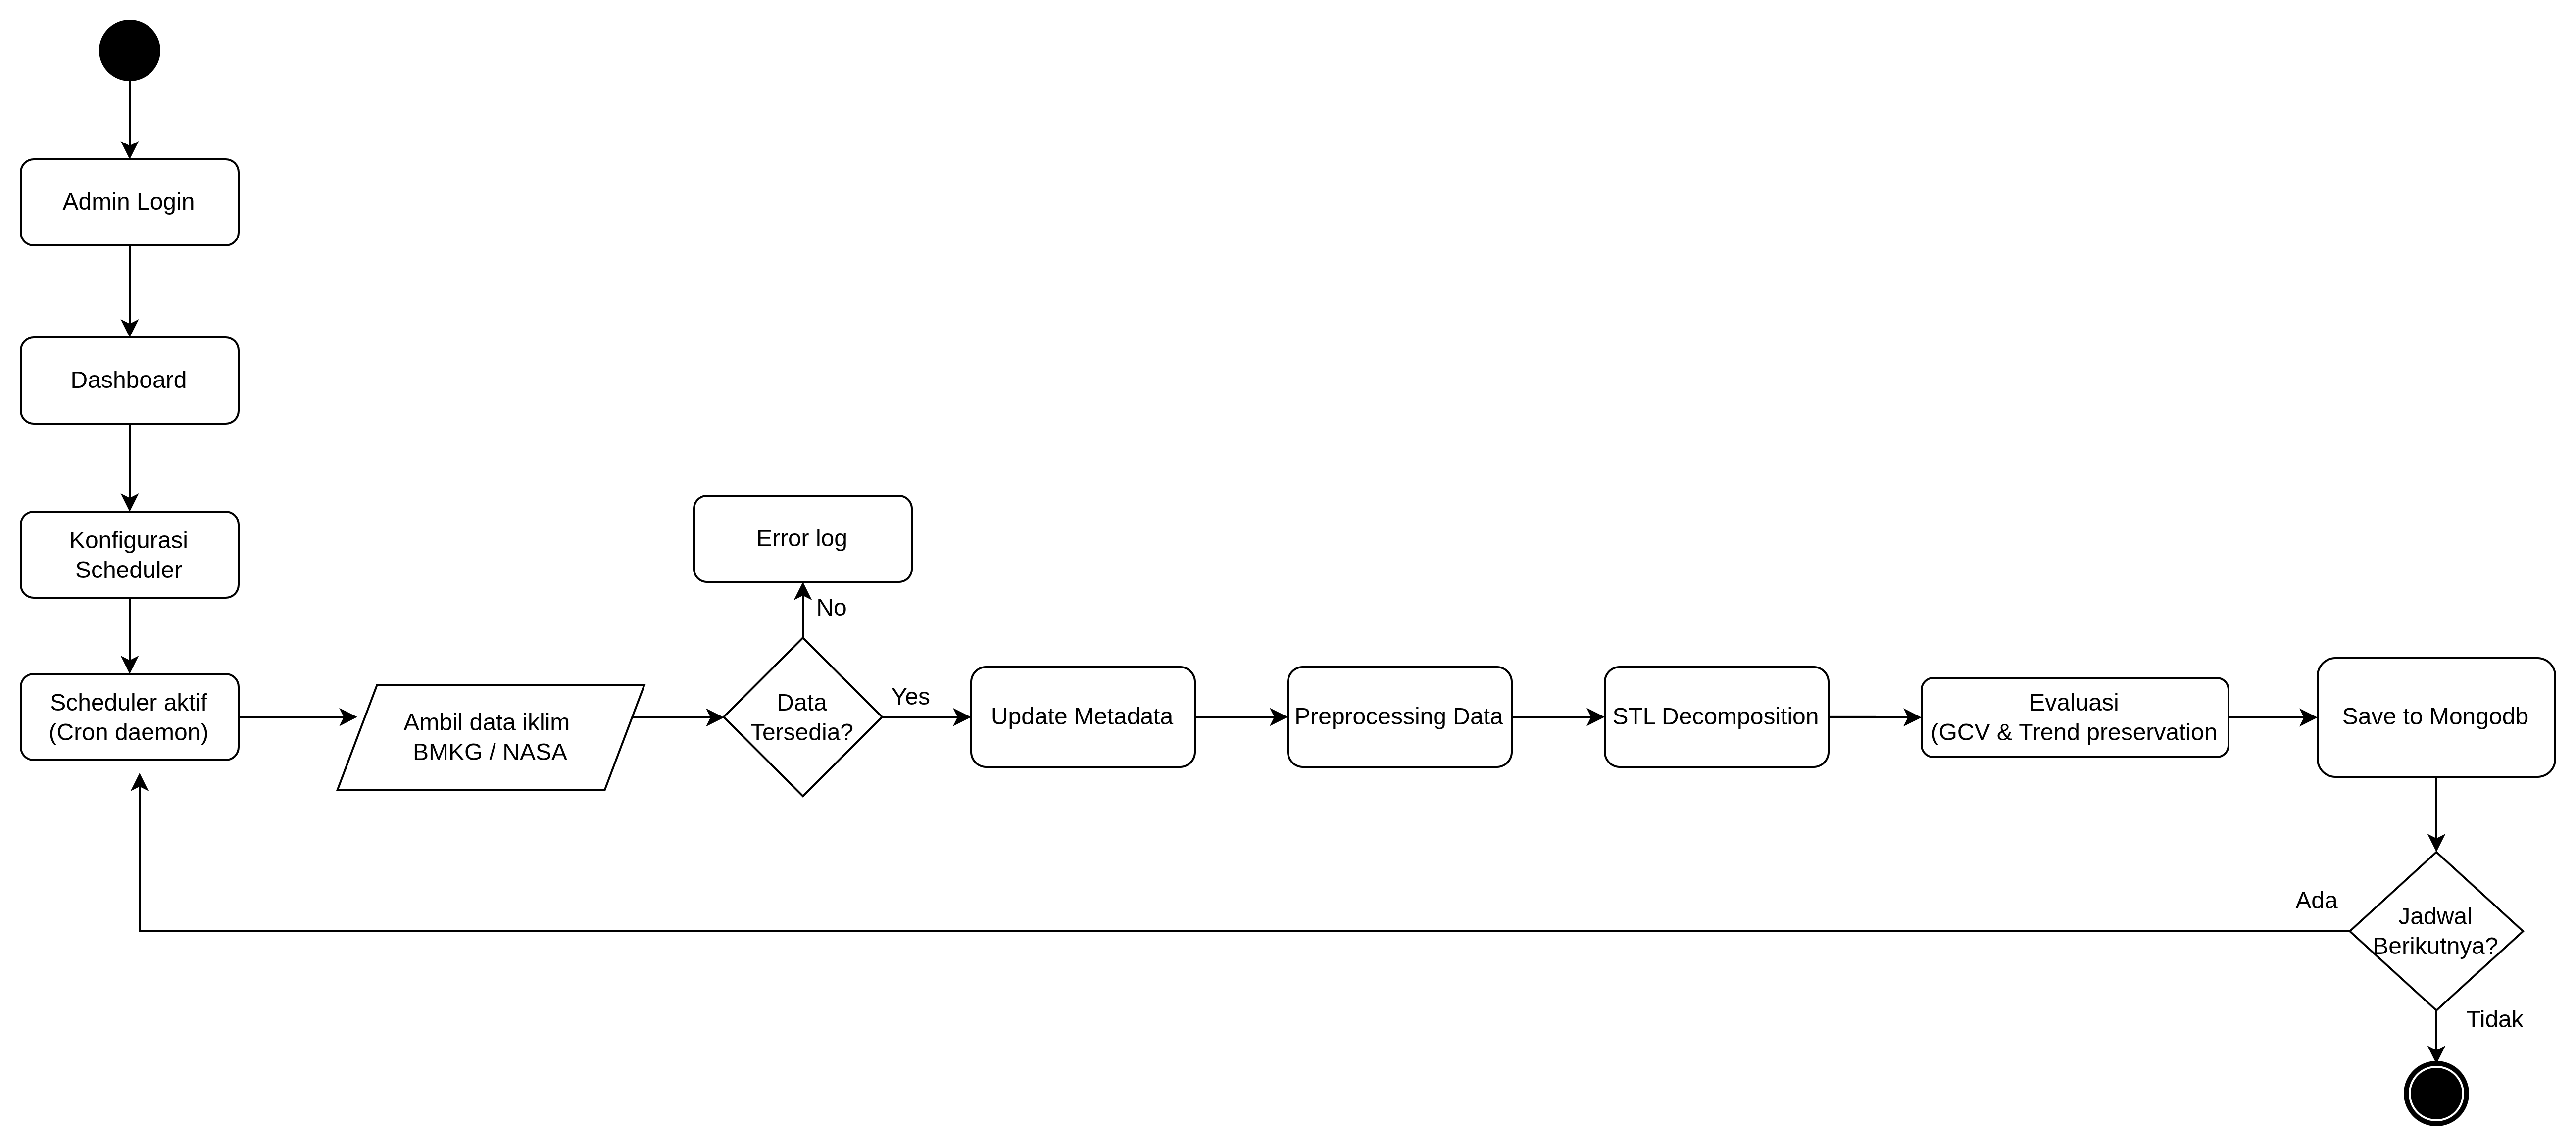
\includegraphics[width=1\linewidth]{image/bab3/flowchart_anggota1.png}
    \caption{\textit{Flowchart} Alur Kerja Anggota 1}
    \label{fig:flowchart_1}
    \end{figure}
    Berdasarkan Gambar \ref{fig:flowchart_1}, proses diawali dengan admin melakukan login ke sistem dan mengakses \textit{dashboard} untuk melakukan konfigurasi \textit{scheduler}. Setelah konfigurasi tersimpan, \textit{cron daemon} akan aktif dan secara otomatis menjalankan proses pengambilan data iklim dari sumber BMKG atau NASA POWER sesuai jadwal yang telah ditentukan. Sistem kemudian memeriksa ketersediaan data yang diperoleh. Jika data tidak tersedia, sistem mencatat kegagalan ke dalam \textit{error log}. Sebaliknya, apabila data tersedia, sistem melakukan pembaruan metadata \textit{dataset} sebelum memasuki tahap \textit{preprocessing} yang mencakup proses pembersihan dan transformasi data. Selanjutnya dilakukan dekomposisi STL (\textit{Seasonal-Trend decomposition using LOESS}) untuk memperoleh komponen tren, musiman, dan residual yang digunakan dalam evaluasi kualitas hasil \textit{preprocessing}. Evaluasi dilakukan menggunakan metrik \textit{Generalized Cross-Validation} dan \textit{trend preservation}. Setelah seluruh proses selesai, \textit{dataset} beserta hasil evaluasinya disimpan ke MongoDB, dan sistem akan menunggu jadwal eksekusi berikutnya sesuai konfigurasi \textit{scheduler}.

    \item \textbf{Perancangan \textit{frontend}}: Membangun rancangan \textit{interface} untuk memantau alur otomasi data. Desain awal dibangun dalam bentuk \textit{high-fidelity prototype}. Tampilan fitur utama yang dirancang adalah halaman (\ref{automasi}).
    \begin{figure}[H]
    \centering
    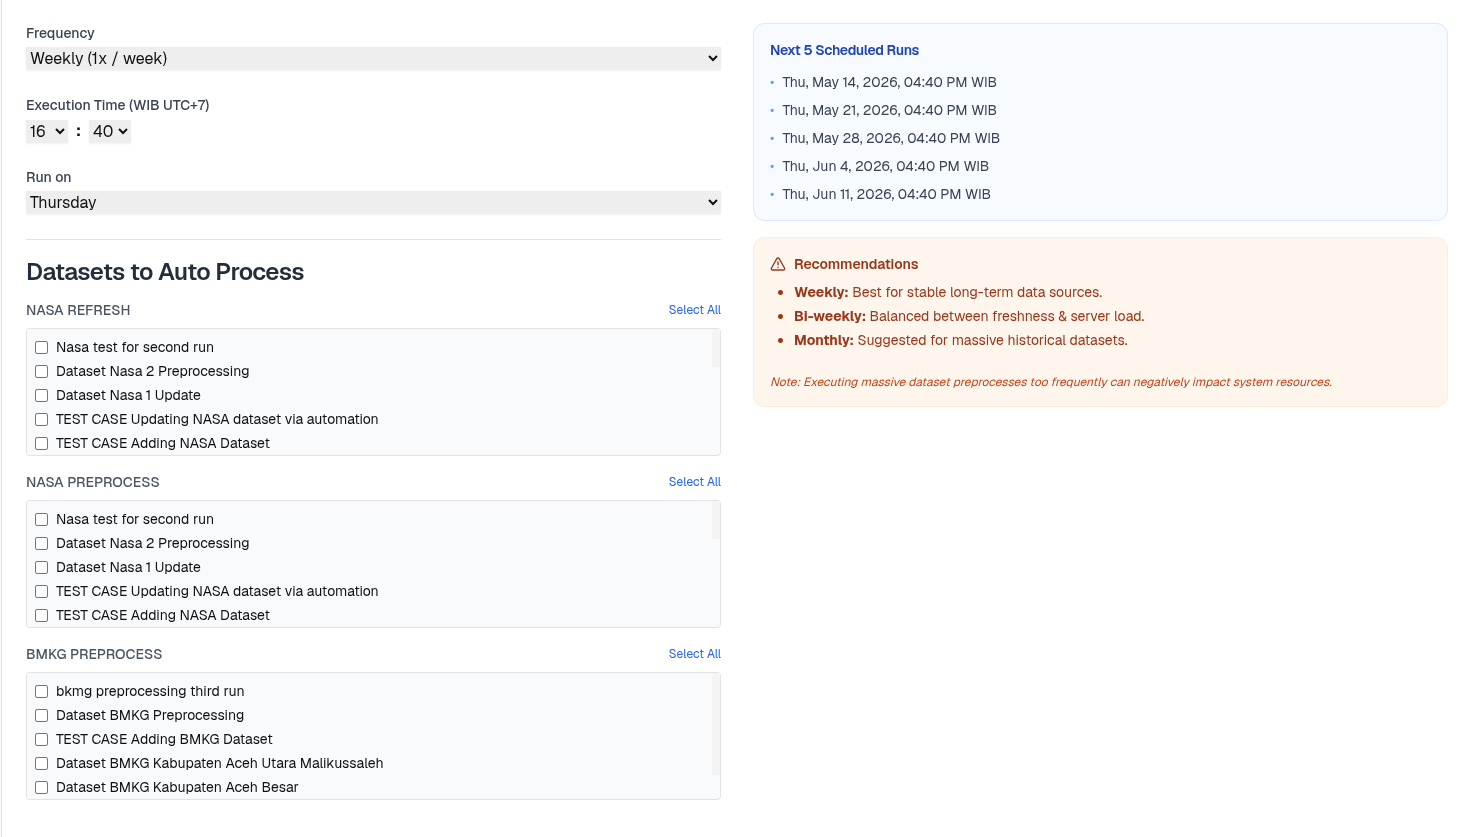
\includegraphics[width=1\linewidth]{image/bab3/halaman_otomasi.png}
    \caption{Halaman Otomasi}
    \label{automasi}
    \end{figure}
    \begin{figure}[H]
    \centering
    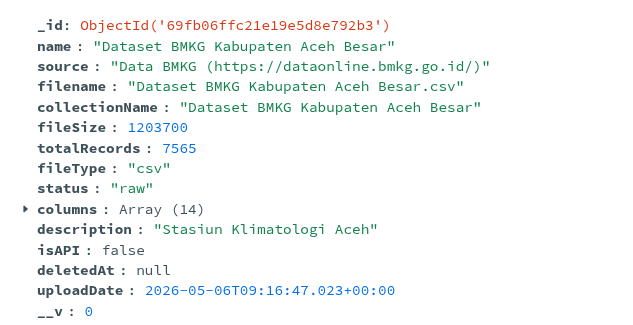
\includegraphics[width=0.8\linewidth]{image/bab3/mongo_metadataset.png}
    \caption{Parameter Metadata}
    \label{dataset_meta}
    \end{figure}
    Berdasarkan gambar \ref{dataset_meta} di atas, meta menyimpan informasi setiap \textit{dataset} di MongoDB. Struktur tersebut mencakup nama \textit{dataset}, sumber data, nama \textit{collection} di MongoDB, totalRecords, fileType, status (misalnya raw untuk data mentah), serta columns (daftar variabel iklim yang tersedia). Metadata ini digunakan sistem untuk melacak asal-usul, ukuran, dan status pengolahan data.

    \item \textbf{Perancangan \textit{backend}}: Mengembangkan \textit{RESTful API} menggunakan \textit{framework} Flask dan Next.js agar terkoneksi ke MongoDB untuk \textit{session} autentikasi, penyimpanan data, dan \textit{summary} hasil \textit{preprocessing}. Perancangan dilakukan menggunakan \textit{NoSQL Database Design} untuk menggambarkan hubungan antar \textit{collection}, kemudian dilengkapi dengan \textit{Document Schema Diagram} untuk menjelaskan struktur dokumen yang disimpan pada setiap \textit{collection}.
    \item \textbf{Perancangan \textit{preprocessing pipeline}}: Bagian ini berfokus pada penyusunan \textit{pipeline} pembersihan \textit{dataset} sehingga hasil data dapat dijadwalkan melalui otomasi. Hasil \textit{preprocessing} akan diakses oleh \textit{frontend}.
\end{enumerate}

% \subsection{Integrasi \textit{database}}
% Pada tahap ini, sistem menghubungkan \textit{backend} dengan \textit{database} MongoDB untuk menyimpan dan mengelola data iklim yang telah diproses. Struktur \textit{database} dirancang untuk menampung berbagai parameter cuaca dalam tabel yang terstruktur dengan baik, sehingga memudahkan proses pengambilan data untuk analisis lebih lanjut. Integrasi dilakukan menggunakan MongoDB, yang memungkinkan manipulasi database dengan lebih efisien dalam lingkungan Next.js. Dilakukan optimasi \textit{query} agar sistem dapat menangani jumlah data yang besar dengan performa yang tetap optimal.

\subsection{Pengujian sistem}
Dilakukan pengujian untuk memastikan setiap komponen dalam \textit{pipeline} berjalan sesuai spesifikasi teknis. Pengujian dilakukan dalam dua aspek utama, diantaranya:

\begin{enumerate}
    \item \textbf{\textit{Integration Testing}} \\
    Pengujian ini dilakukan untuk memastikan seluruh komponen sistem dapat saling berkomunikasi, dimulai dari validasi aliran data mulai dari pengambilan data eksternal, proses \textit{preprocessing}, pengelolaan data pada \textit{frontend}, hingga penyimpanan ke MongoDB. Pada pengujian inilah dipastikan otomasi dapat berjalan sesuai jadwal tanpa kegagalan. Skema pengujian dijabarkan ke dalam skenario Tabel \ref{tab:integration_scenario} berikut.
        \begin{table}[H]
        \centering
        \caption{Skenario Pengujian RESTful API Sistem}
        \label{tab:integration_scenario}
        \scriptsize % Mengecilkan seluruh font tabel
        \setlength{\tabcolsep}{2pt} % Menipiskan jarak antar kolom
        \renewcommand{\arraystretch}{1.1} % Mengatur kerapatan baris
        \begin{tabular}{|c|l|c|c|p{4.2cm}|}
        \hline
        \textbf{No} & \textbf{Endpoint} & \textbf{Meth} & \textbf{Srv} & \textbf{Output Diharapkan} \\ \hline
        1 & \texttt{/api/v1/dataset-meta/} & POST & Next.js & Metadata \& \textit{raw data} tersimpan ke DB \\ \hline
        2 & \texttt{/api/v1/check-mongodb} & GET & Flask & Status \textit{active connection} DB \\ \hline
        3 & \texttt{/api/v1/nasa-power/save} & POST & Next.js & Fetch API NASA \& inisialisasi dataset baru \\ \hline
        4 & \texttt{/api/v1/nasa-power/refresh/:id} & POST & Next.js & Pembaruan data NASA (\textit{new records}) \\ \hline
        5 & \texttt{/api/v1/preprocess/bmkg/:name} & POST & Flask & \textit{Cleaned dataset} \& \textit{preprocessing report} \\ \hline
        6 & \texttt{/api/v1/preprocess/nasa/.../stream} & GET & Flask & Eksekusi STL \textit{Decomposition} via SSE \textit{stream} \\ \hline
        7 & \texttt{/api/v1/preprocess/bmkg/.../stream} & GET & Flask & Eksekusi STL \textit{Decomposition} via SSE \textit{stream} \\ \hline
        8 & \texttt{/api/v1/scheduler/config} & POST & Flask & Konfigurasi otomasi \& \textit{daemon} \textit{cron} tersimpan \\ \hline
        9 & \texttt{/api/v1/scheduler/trigger} & POST & Flask & Memicu eksekusi \textit{worker} (Manual/Quick) \\ \hline
        10 & \texttt{/api/v1/dataset-meta/:name/delete} & PATCH & Next.js & \textit{Soft delete} (update field \texttt{deletedAt}) \\ \hline
        11 & \texttt{/api/v1/dataset-meta/:name} & DELETE & Next.js & \textit{Cascade delete} (Data \& reports bersih) \\ \hline
        \end{tabular}
        \end{table}
    Tabel \ref{tab:integration_scenario} merincikan skenario pengujian RESTful API yang mencakup \textit{endpoint} untuk integrasi fungsi spesifik. Contohnya koneksi \textit{database}, pembaruan data, proses \textit{preprocessing}, dan penjadwalan otomasi.

    \item \textbf{Pengujian Kualitas Data} \\
    Evaluasi kualitas hasil \textit{preprocessing} dilakukan menggunakan dua metrik utama, yaitu GCV dan \textit{trend preservation}. GCV digunakan untuk memilih parameter \textit{smoothing} optimal dengan menyeimbangkan antara \textit{goodness of fit} dan kompleksitas model, di mana nilai GCV minimum menunjukkan parameter \textit{smoothing} terbaik.

    Selain GCV, evaluasi juga mempertimbangkan kemampuan metode dalam mempertahankan pola tren dengan \textit{trend preservation}. Pengujian ini dilakukan dengan membandingkan kesesuaian pola tren antara data sebelum dan sesudah \textit{preprocessing} melalui dekomposisi STL. Evaluasi ini bertujuan memastikan bahwa proses imputasi maupun \textit{smoothing} tidak menghilangkan karakteristik utama data iklim, seperti kecenderungan naik-turun musiman dan perubahan jangka panjang.

\end{enumerate}
\begin{comment}
\end{comment}
